\section{Evaluation}
\label{sec:evaluation}
We evaluate the performance of our solution on a single general purpose
Amazon EC2 m3.large instance, running Debian 8.3 (Jessie)
and equipped with an Intel Xeon E5-2670 v2 (Ivy Bridge)  (2.6 GHz,
8 cores and 20 MB cache), 7.5 GB of RAM and a general purpose SSD.
%
The experimental framework consists in evaluating the perfromance achieved by Ontoqa in terms of response-time.
%
The input considered in experimentations are questions caracterized by distinct complexities, in terms of structure and ambiguities.

\begin{figure}[H]
	\centering
	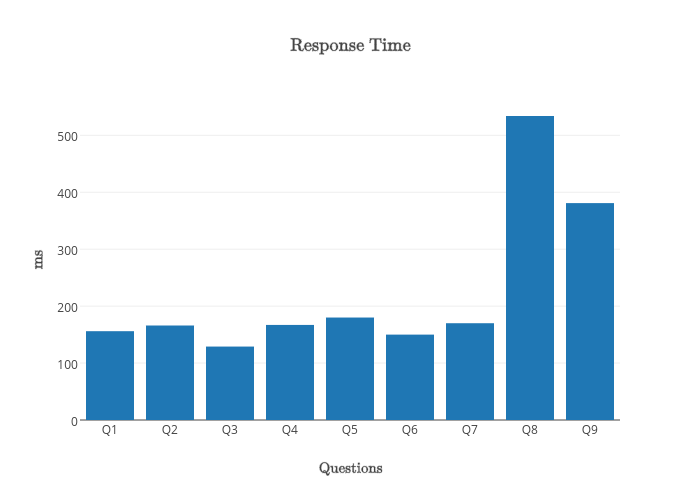
\includegraphics[width=0.8\columnwidth]{./fig/evaluation-response-time}
	\caption{Respinse time performance of Ontoqa on the benchmark questions.}
	\label{fig:evaluation-response-time}
\end{figure}

In particular we examine the following class of questions:

\begin{itemize}
	\item[Q1] questions in the form \textit{'who founded Microsoft?'}.
	\item[Q2] questions in the form \textit{'who are the corporate officers of Microsoft?'}.
	\item[Q3] questions in the form \textit{'where is Microsoft headquartered?'}.
	\item[Q4] questions in the form \textit{'what is the most valuable company?'}.
	\item[Q5] questions in the form \textit{'who are the corporate officers of the most valuable company?'}.
	\item[Q6] questions in the form \textit{'is Satya Nadella the CEO of Microsoft?'}.
	\item[Q7] questions in the form \textit{'did Microsoft acquire a company headquartered in Italy?'}.
	\item[Q8] questions in the form \textit{'is Satya Nadella italian?'}.
	\item[Q9] questions in the form \textit{'did Microsoft acquire an italian company?'}.
\end{itemize}

Notice that questions \texttt{Q1-Q7} do not induce any semantic ambiguity, while questions \texttt{Q8} and \texttt{Q9} do due to the presence of the entry \textit{'italian'}. In fact, the latter can be referred both to companies (e.g. a company headquartered in Italy) and to people (e.g. a person with italian nationality).
%
The experiments have been carried out by averaging measurements on randomly ordered 10 executions.
%
Figure~\ref{fig:evaluation-response-time} shows, the \textit{response time} achieved by Ontoqa when facing with the benchmark questions \texttt{Q1}-\texttt{Q8}.
%
The former has been measured considering the time elapsed for the question to be answered, calling the Java built-in function \texttt{System.currentTimeMillis()}.

The results are coherent with the theoretical and implementation framework. In fact, we can observe that (i) unambiguous questions (\texttt{Q1-Q7}) induce a response time proportional to the depth of the generated LTAG and (ii) the questions involving ambiguities (\texttt{Q8 and Q9}) induce a response time proportional to the complexity of the ambiguity.